\subsection{UC6 - Ricerca documentale}
\begin{itemize}
    \item \textbf{Identificativo}: UC6
    \item \textbf{Nome}: ricerca documentale
    \item \textbf{Descrizione grafica}:
\end{itemize}

\begin{figure}[h]
   \centering
   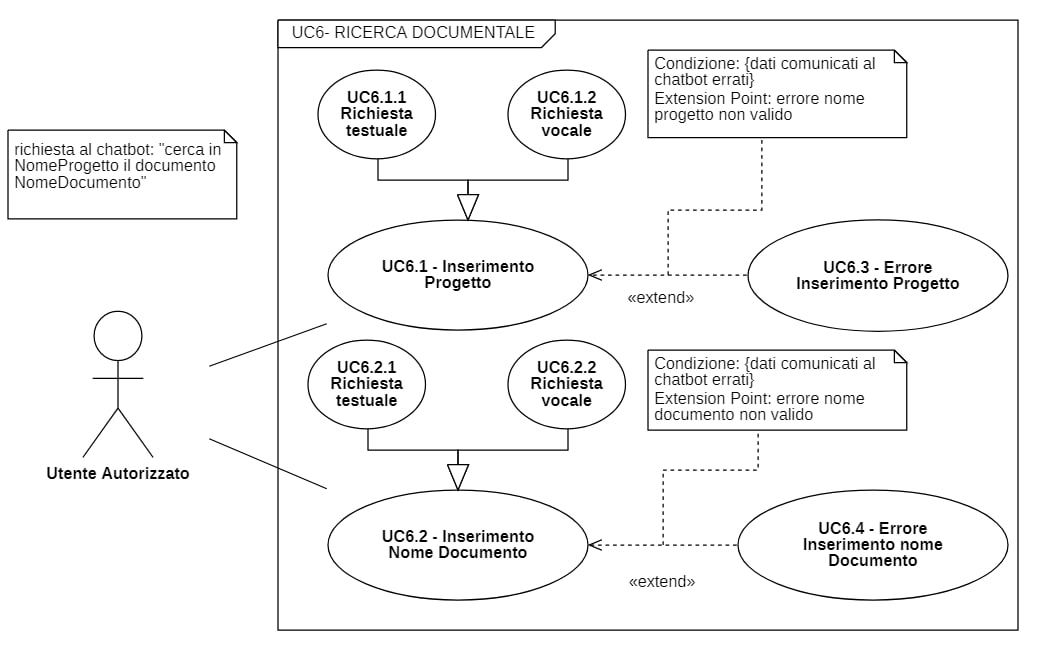
\includegraphics[scale=2]{images/UC6.png} 
   \caption{Descrizione grafica caso d'uso UC6}
\end{figure}

 \begin{itemize}
    \item \textbf{Attori}
 \begin{itemize} 
    \item \textit{Primari}: utente autorizzato
    \item \textit{Secondari}: non presenti
 \end{itemize}
 \item \textbf{Precondizione}: l'utente è autorizzato e si trova nell'interfaccia del chatbot.
 \item \textbf{Postcondizione}: il chatbot risponde alla richiesta dell'utente mostrando i documenti trovati.
 \item \textbf{Scenario principale}: l'utente autorizzato chiede al chatbot la ricerca di documenti, specificando il progetto al quale è associato (UC6.1) e il nome del documento (UC6.2).
 \item \textbf{Estensioni}: 
 \begin{itemize} 
    \item il chatbot comunica all'utente che l'inserimento del nome del progetto (UC6.3) o del nome del documento (UC6.4) non sono corretti.
 \end{itemize}
\end{itemize}
\newpage
\subsubsection{UC6.1 - Inserimento progetto}
\begin{itemize}
    \item \textbf{Identificativo}: UC6.1
    \item \textbf{Nome}: inserimento progetto
    \item \textbf{Descrizione grafica}: (approfondita in UC6)
    \item \textbf{Attori}
 \begin{itemize} 
    \item \textit{Primari}: utente autorizzato
    \item \textit{Secondari}: non presenti
 \end{itemize}
 \item \textbf{Precondizione}: l'utente ha richiesto al chatbot la ricerca di un documento.
 \item \textbf{Postcondizione}:  l'utente ha comunicato al chatbot il progetto nel quale ricercare i documenti.
 \item \textbf{Scenario principale}: il chatbot chiede all'utente di specificare il progetto nel quale ricercare i documenti. L'utente comunica al chatbot il progetto tramite messaggio testuale (UC6.1.1) o vocale (UC6.1.2).
 \item \textbf{Estensioni}: 
 \begin{itemize} 
    \item il chatbot comunica all'utente che il nome del progetto inserito non è corretto (UC6.3).
 \end{itemize}
\end{itemize}

\paragraph{UC6.1.1 - Richiesta Testuale}
\begin{itemize}
   \item \textbf{Identificativo}: UC6.1.1
   \item \textbf{Nome}: Richiesta testuale
   \item \textbf{Descrizione grafica}: (approfondita in UC6)
   \item \textbf{Attori}:
   \begin{itemize} 
       \item \textit{Primari}: utente autorizzato
       \item \textit{Secondari}: non presenti
   \end{itemize}
       \item \textbf{Precondizione}: l'utente si è autenticato al sistema e ha richiesto di voler cercare un documento all'interno di un progetto.
       \item \textbf{Postcondizione}: l'utente fornisce il nome del progetto in maniera testuale
    \item \textbf{Scenario principale}: 
       \begin{itemize}
           \item L'utente ha effettuato l'accesso al sistema 
           \item L'utente fornisce tramite input testuale il nome del progetto su cui fare la ricerca del documento
       \end{itemize}
\end{itemize}

\paragraph{UC6.1.2 - Richiesta Vocale}
\begin{itemize}
   \item \textbf{Identificativo}: UC6.1.2
   \item \textbf{Nome}: Richiesta vocale
   \item \textbf{Descrizione grafica}: (approfondita in UC6)
   \item \textbf{Attori}:
   \begin{itemize} 
       \item \textit{Primari}: utente autorizzato
       \item \textit{Secondari}: non presenti
   \end{itemize}
       \item \textbf{Precondizione}: l'utente si è autenticato al sistema e ha richiesto di voler cercare un documento all'interno di un progetto.
       \item \textbf{Postcondizione}: l'utente fornisce il nome del progetto in maniera vocale
    \item \textbf{Scenario principale}: 
       \begin{itemize}
           \item L'utente ha effettuato l'accesso al sistema 
           \item L'utente fornisce tramite input vocale il nome del progetto su cui fare la ricerca del documento
       \end{itemize}
\end{itemize}

\subsubsection{UC6.2 - Inserimento nome documento}
\begin{itemize}
    \item \textbf{Identificativo}: UC6.2
    \item \textbf{Nome}: inserimento nome documento
    \item \textbf{Descrizione grafica}: (approfondita in UC6)
    \item \textbf{Attori}
 \begin{itemize} 
    \item \textit{Primari}: utente autorizzato
    \item \textit{Secondari}: non presenti
 \end{itemize}
 \item \textbf{Precondizione}: l'utente ha richiesto al chatbot la ricerca di un documento.
 \item \textbf{Postcondizione}:  l'utente ha comunicato al chatbot il nome del documento da ricercare.
 \item \textbf{Scenario principale}: il chatbot chiede all'utente di specificare il nome del documento da ricercare. L'utente comunica al chatbot il nome del documento tramite messaggio testuale (UC6.1.1) o vocale (UC6.1.2).
 \item \textbf{Estensioni}: 
\begin{itemize} 
    \item il chatbot comunica all'utente che il nome del documento inserito non è corretto (UC6.4).
 \end{itemize}
\end{itemize}

\paragraph{UC6.2.1 - Richiesta Testuale}
\begin{itemize}
   \item \textbf{Identificativo}: UC6.2.1
   \item \textbf{Nome}: Richiesta testuale
   \item \textbf{Descrizione grafica}: (approfondita in UC6)
   \item \textbf{Attori}:
   \begin{itemize} 
       \item \textit{Primari}: utente autorizzato
       \item \textit{Secondari}: non presenti
   \end{itemize}
       \item \textbf{Precondizione}: l'utente si è autenticato al sistema e ha richiesto di voler cercare un documento all'interno di un progetto.
       \item \textbf{Postcondizione}: l'utente fornisce il nome del documento in maniera testuale
    \item \textbf{Scenario principale}: 
       \begin{itemize}
           \item L'utente ha effettuato l'accesso al sistema 
           \item L'utente fornisce tramite input testuale il nome del documento da ricercare
       \end{itemize}
\end{itemize}

\paragraph{UC6.2.2 - Richiesta Vocale}
\begin{itemize}
   \item \textbf{Identificativo}: UC6.2.2
   \item \textbf{Nome}: Richiesta vocale
   \item \textbf{Descrizione grafica}: (approfondita in UC6)
   \item \textbf{Attori}:
   \begin{itemize} 
       \item \textit{Primari}: utente autorizzato
       \item \textit{Secondari}: non presenti
   \end{itemize}
       \item \textbf{Precondizione}: l'utente si è autenticato al sistema e ha richiesto di voler cercare un documento all'interno di un progetto.
       \item \textbf{Postcondizione}: l'utente fornisce il nome del documento in maniera vocale
    \item \textbf{Scenario principale}: 
       \begin{itemize}
           \item L'utente ha effettuato l'accesso al sistema 
           \item L'utente fornisce tramite input vocale il nome del documento da ricercare
       \end{itemize}
\end{itemize}

\subsubsection{UC6.3 - Errore inserimento nome progetto}
\begin{itemize}
    \item \textbf{Identificativo}: UC6.3
    \item \textbf{Nome}: errore inserimento nome progetto
    \item \textbf{Descrizione grafica}: (approfondita in UC6)
    \item \textbf{Attori}
 \begin{itemize} 
    \item \textit{Primari}: utente autorizzato
    \item \textit{Secondari}: non presenti
 \end{itemize}
 \item \textbf{Precondizione}: l'utente ha inserito un nome di progetto non valido.
 \item \textbf{Postcondizione}:  il chatbot comunica all'utente che il nome di progetto specificato non è corretto.
 \item \textbf{Scenario principale}: il chatbot comunica all'utente l'errore nell'inserimento del nome di progetto e chiede di reinserirlo.
\end{itemize}
\subsubsection{UC6.4 - Errore inserimento nome documento}
\begin{itemize}
    \item \textbf{Identificativo}: UC6.4
    \item \textbf{Nome}: errore inserimento nome documento
    \item \textbf{Descrizione grafica}: (approfondita in UC6)
    \item \textbf{Attori}
 \begin{itemize} 
    \item \textit{Primari}: utente autorizzato
    \item \textit{Secondari}: non presenti
 \end{itemize}
 \item \textbf{Precondizione}: l'utente ha inserito un nome documento non valido.
 \item \textbf{Postcondizione}:  il chatbot comunica all'utente che il nome del documento specificato non è corretto.
 \item \textbf{Scenario principale}: il chatbot comunica all'utente l'errore nell'inserimento del nome del documento e chiede di reinserirlo.
\end{itemize}
\newpage